\documentclass[dvipdfmx,10pt,fleqn,a4paper,twocolumn]{jsarticle}
\usepackage{graphicx,color}
\usepackage[margin=15truemm]{geometry}
\usepackage{ascmac,amsmath,amssymb,array}
\usepackage{tikz}
\usetikzlibrary{calc,angles,quotes,intersections}
\usepackage{surikumi-patterns-platex}
\usepackage{zogeny,ceo,cuted}
\usepackage{thick-itembox}%太いitembox
\usepackage[haranoaji]{pxchfon}
\usepackage[fontsize=8.5pt]{fontsize}
\renewcommand{\baselinestretch}{1.3}
\newcommand{\midashikakko}[1]{《#1》}%ダブルのカギカッコ
\newcommand{\ans}[1]{\mbox{\boldmath{$#1$}}}

\newcommand{\dotshiki}[2]{%
  \begin{equation*}
    \hbox to \dimexpr\linewidth-\mathindent\relax{%
      \mathsurround=0pt
      $\displaystyle #1$%
      \kern.5em
      \cleaders\hbox{$\mkern1mu\cdot\mkern1mu$}\hfill
      \kern.3em
      \ensuremath{#2}%
    }%
  \end{equation*}%
}%cdots と式番号をページの端まで自動で引く
\makeatletter
\newcommand{\dotshikialign}[2]{%
  \notag
  \ifmeasuring@
    #1\quad\ensuremath{#2}%
  \else
    \hbox to \dimexpr
      \displaywidth-\eqnshift@-\maxcol@width1\relax{%
      \mathsurround=0pt
      $\displaystyle{}#1$%
      \kern.5em
      \cleaders\hbox{$\mkern1mu\cdot\mkern1mu$}\hfill
      \kern.3em
      \ensuremath{#2}%
    }%
  \fi
}
\makeatother%align 環境内でのcdots と式番号をページの端まで自動で引く
\newcommand{\dotshikicenter}[2]{%
  \par\begingroup
  \mathsurround=0pt
  \setbox0=\hbox{$\displaystyle #1$}%
  \dimen0=\dimexpr(\linewidth-\wd0)/2\relax
  \noindent\hbox to\linewidth{%
    \kern\dimen0
    \box0
    \kern.5em
    \cleaders\hbox{$\mkern1mu\cdot\mkern1mu$}\hfill
    \kern.3em
    \ensuremath{#2}%
  }\par
  \endgroup
}

\newcommand{\hokuban}[1]{
\begin{tikzpicture}[scale=1]
\filldraw[fill=black,draw=black](0,0)--({1-0.2},{0})--({1-0.2},{1-0.2})--(0,{1-0.2})--(0,0);
\draw[-,thick](0,0)--({1-0.2},{0})--({1/2-0.2},{1-0.2})--(0,{1-0.2})--(0,0);
\node[white,font=\Huge]at({1/2-0.1},{1/2-0.1})(label){$\mathbf{#1}$};
\end{tikzpicture}}%全国大学入試問題のでかい「問題番号」
% 「解答」記号は初回だけTikZで作り、以後は同じボックスを再利用する。

\newsavebox{\hokuikaibasebox}
\newcommand{\hokukai}{%
  \ifvoid\hokuikaibasebox
    \global\setbox\hokuikaibasebox=\hbox{%
      \begin{tikzpicture}[baseline=(kaitext.base)]
        \draw[line width=0.2mm](-0.6,{-1/5+0.04})--(-0.6,{1/5-0.03})--(0.6,{1/5-0.03})--(0.6,{-1/5+0.04})--cycle;
        \draw[line width=0.5mm](-0.6,{-1/5+0.03})--(-0.6,{1/5-0.02});
        \draw[line width=0.5mm](0.6,{-1/5+0.03})--(0.6,{1/5-0.02});
        \node at(0,0){\kurosankakub \ans{解答}\kurosankakua};
        \node (kaitext) at (0,0){\kurosankakub \ans{解答}\kurosankakua};
      \end{tikzpicture}%
    }%
  \fi
  \usebox{\hokuikaibasebox}%
} %全国大学入試問題の「解答」記号

\newcommand{\theme}[1]{【\text{#1}】}

\newcommand{\KTileGlyph}[2]{%
  \foreach \dx/\dy in {
    -.16/0,.16/0,0/-.16,0/.16,
    -.11/-.11,-.11/.11,.11/-.11,.11/.11,0/0
  }{%
    \node[inner sep=0pt,text=#1,
      font=\gtfamily\fontseries{bx}\fontsize{34}{34}\selectfont]
      at ({7+\dx},{6.65+\dy}) {#2};
  }%
}
\newcommand{\KTileWhite}[2]{%
  \begin{scope}[shift={(#1,0)}]
    \path[fill=white,draw=black,line width=1.05mm,
      rounded corners=1.35mm]
      (1.25,-1.25) rectangle (15.25,12.75);
    \draw[black,line width=1.05mm,line cap=round]
      (14,14)--(15.25,12.75);
    \draw[black,line width=1.05mm,line cap=round]
      (0,0)--(1.25,-1.25);
    \path[fill=white,draw=black,line width=1.05mm,
      rounded corners=1.35mm]
      (0,0) rectangle (14,14);
    \KTileGlyph{black}{#2}
  \end{scope}%
}
\newcommand{\KTileBlack}[2]{%
  \begin{scope}[shift={(#1,0)}]
    \path[fill=white,draw=black,line width=1.05mm,
      rounded corners=1.35mm]
      (1.25,-1.25) rectangle (15.25,12.75);
    \draw[black,line width=1.05mm,line cap=round]
      (14,14)--(15.25,12.75);
    \draw[black,line width=1.05mm,line cap=round]
      (0,0)--(1.25,-1.25);
    \path[fill=black,draw=black,line width=1.05mm,
      rounded corners=1.35mm]
      (0,0) rectangle (14,14);
    \draw[white,line width=.45mm,rounded corners=.85mm]
      (.85,.85) rectangle (13.15,13.15);
    \KTileGlyph{white}{#2}
  \end{scope}%
}
\newsavebox{\hokukanbasebox}
\newcommand{\hokukan}[1][11.6mm]{%
  \ifvoid\hokukanbasebox
    \global\setbox\hokukanbasebox=\hbox{%
      \begin{tikzpicture}[x=1mm,y=1mm]
        \KTileWhite{0}{考}
        \KTileBlack{17.65}{え}
        \KTileWhite{35.30}{方}
      \end{tikzpicture}%
    }%
  \fi
  \raisebox{-.4ex}{%
    \resizebox{#1}{!}{\usebox{\hokukanbasebox}}%
  }%
}%ほくそむの考え方記号
% 別解：既存の \KTileWhite・\KTileBlack を使用
\newsavebox{\hokubekkaibasebox}
\newcommand{\hokubekkai}[1][8.3mm]{%
  \ifvoid\hokubekkaibasebox
    \global\setbox\hokubekkaibasebox=\hbox{%
      \begin{tikzpicture}[x=1mm,y=1mm]
        \KTileWhite{0}{別}
        \KTileBlack{18.65}{解}
      \end{tikzpicture}%
    }%
  \fi
  \raisebox{-.4ex}{%
    \resizebox{#1}{!}{\usebox{\hokubekkaibasebox}}%
  }%
}
\setlength{\parindent}{0pt}
\tikzset{geom/.style={line width=.65pt,line cap=round,line join=round,font=\small},
  aux/.style={densely dashed,line width=.45pt},
  every pic/.style={draw,angle radius=4mm,angle eccentricity=1.5}}
\newcommand{\pt}[2]{\fill (#1) circle(1.2pt) node[#2,inner sep=2pt]{$#1$};}
\newcommand{\Head}[2]{\par\noindent\ba{#1}.\quad{\large\gtfamily\fontseries{bx}\selectfont #2}\par\vspace{3mm}}
\newcommand{\Sub}[1]{\par\vspace{2mm}\noindent{\gtfamily\fontseries{bx}\selectfont #1}\par\vspace{1mm}}
\newcommand{\Note}[1]{\par\vspace{1mm}{\small\chu\quad #1}\par}
\newcommand{\GeoRow}[2]{%
  \par\vspace{1mm}\noindent
  \begin{minipage}[c]{.59\linewidth}#1\end{minipage}\hfill
  \begin{minipage}[c]{.37\linewidth}\centering #2\end{minipage}
  \par\vspace{2mm}}
\newlength{\PatternTitleHeight}
\setlength{\PatternTitleHeight}{28mm}
\makeatletter
\newcommand{\PatternTitle}[5][kagome]{%
  \par\addvspace{1.2\baselineskip}\begingroup
  \SurikumiPatternSetup{pattern=#1,pattern-tone=normal}%
  \noindent\begin{tikzpicture}
    \path[use as bounding box](0,0) rectangle (\linewidth,\PatternTitleHeight);
    \path[fill=SMpale](0,0) rectangle (\linewidth,\PatternTitleHeight);
    \smag@patternfill{0}{0}{\linewidth}{\PatternTitleHeight}
    \draw[draw=SMrule,line width=.45pt](0,0) rectangle (\linewidth,\PatternTitleHeight);
    \node[anchor=north west,xshift=3mm,yshift=-2.2mm,inner sep=0pt,
      font=\sffamily\gtfamily\bfseries\small] at (0,\PatternTitleHeight)
      {#2\hspace{.8em}\rule[-.15ex]{.45pt}{1.25em}\hspace{.8em}#3};
    \node[fill=white,inner sep=4pt,font=\sffamily\gtfamily\bfseries\LARGE]
      at (.5\linewidth,.5\PatternTitleHeight){#4};
    \node[anchor=south east,xshift=-3mm,yshift=2mm,inner sep=0pt,
      font=\gtfamily\scriptsize] at (\linewidth,0){#5};
  \end{tikzpicture}\par\endgroup\vspace{3mm}}%大数の題名
\makeatother
\setlength{\columnsep}{25pt}
\begin{document}
\twocolumn[{%
\PatternTitle[weave]{演習}{数学III}{微積の周辺}{大島　遙斗}
\kurosankakub 微積分の周辺,具体的には（極限・微分・数式における積分・面積・体積）です.基礎的な解法・考え方については新数学スタンダード演習でかなり
定着することができたと思っているので,ここでは入試標準から応用レベルの大切な問題を扱います.\kurosankakua}\vspace{5mm}]
{\Large\ans{1章}\quad \ans{同次式}}\\
同次式とは,次のような形のものを言う.
\begin{itembox}
[l]{\enpitu 定義}
関数$z=\dfrac{f(x)}{g(x)}$について,
\begin{center}
$\deg{f(x)}=\deg{g(x)}$
\end{center}のとき,
$z$を同次式と言う.ここで,$\deg f(x)$は,$f(x)$の次数である.\\
すなわち,「分母と分子の次数が等しい」ということである.
\end{itembox}
同次式の解法は決まっている.次の例題を挙げて考えてみよう.\\
\reidaic\quad$x,y$が正の実数全体を動くとき,$z=\dfrac{xy+x^2+y^2}{x^2+xy}$の最小値を求めよ.\\
\hokukan\quad 2変数関数なのが嫌なので,どうにか変数を減らすことを考えましょう.$x^2$か$y^2$で分母・分子を割ると良さそうですね.\\
\hokukai\quad $z$の分母・分子を$x^2$で割ると,
\begin{align*}
  z&=\dfrac{\frac{y}{x}+1+\p{\frac{y}{x}}^2}{1+\frac{y}{x}}\\
  &=\dfrac{t^2+t+1}{1+t}\quad（\temarkua\quad t=\frac{y}{x} とおいた.）\\
  &=\dfrac{\p{t+1}^2-t}{t+1}\quad（\temarkua\quad 頭でっかちは次数下げ）\\
  &=t+1-\dfrac{t+1-1}{t+1}\\
  &=\dotshikialign{t+\dfrac{1}{t+1}}{\maruichi}
\end{align*}
$\maruichi$から最小値を求める方法は様々です.\\
\ans{1}.\ans{AM-GMを使う}
\begin{align*}
  \maruichi\doti z=t+1+\dfrac{1}{t+1}-1
\end{align*}
より,$t>0$なので,AM-GMの関係を用いると,
\begin{align*}
  z&=t+1+\dfrac{1}{t+1}-1\\
  &\geq2\sqrt{\p{t+1}\cdot\dfrac{1}{t+1}}-1\\
  &=1
\end{align*}
等号成立は,
\begin{align*}
  t+1=\dfrac{1}{t+1}\doti t=0
\end{align*}
で成立するので,求める最小値は,\ans{1}\\\\
\ans{2.微分する}\\
$\maruichi$において,$z$を$t$の関数とみて,微分すると,
\begin{align*}
  z^\prime&=1-\dfrac{1}{(t+1)^2}\\
  &=\dfrac{t(t+2)}{(t+1)^2}
\end{align*}
よって,次の増減表を得る.
\begin{center}
  \begin{tabular}{|c||c|c|c|c|c|}
    \hline
    $t$&$\cdots$&$-2$&$\cdots$&0&$\cdots$\\
    \hline
    $z^\prime(t)$&$+$&0&$-$&0&$+$\\
    \hline
    $z$&$\yaa$&{}&$\yab$&1&$\yaa$\\
    \hline
  \end{tabular}
\end{center}
よって,$z$の最小値は,\ans{1}\\\\
\ans{3.軌跡の考え方}\\
$z$の値域を$W$とおく.$z=\dfrac{t^2+t+1}{t+1}$において,$z=k$おくと,
\begin{align*}
  k\in W&\doti\exists t, k=\dfrac{t^2+t+1}{t+1}\\
  &\doti \exists t,t^2+(1-k)t+1-k=0\cdots\cdots\maruni\\
  &\doti\maruni を満たす正の実数tが少なくとも一つ存在する.\\
  &\doti（\maruni の判別式：）\p{1-k}^2-4\p{1-k}\geq0\\
  &\doti\p{k+3}\p{k-1}\geq0\\
  &\doti k\geq1\quad（\because k>0）
\end{align*}
よって,$z$の最小値は,\ans{1}\\
\theme{\ans{同次式の扱い方}}
\begin{center}
  \ans{分母と分子を同じ次数で割ればよい!}
\end{center}
ということです.\\それでは,演習問題です.\\\\
\ba{1$\bullet$1}次の問題を解け.\\
\kakkoichi$x,y$が正の実数を動くとき,$z=\dfrac{2x^2+3xy+4y^2}{x^2+y^2}$の最大値を求めよ.\\
\kakkoni$0<x<y$のとき,$z=\dfrac{3x^2y-6xy^2+2y^3}{(x-y)^3}$のとり得る値の範囲を求めよ.\\\\
\ba{1$\bullet$2}\midashikakko{京都大}\\
  $a$は0でない実数とする.
  \begin{align*}
    -\dfrac12\leq\dfrac{x-y}{x+y}\leq\dfrac12
  \end{align*}
  を満たすすべての正の実数$x,y$に対し,
  \begin{align*}
    x^3-3a^2xy^2+2y^3\geq0
  \end{align*}
  が成り立つような$a$の範囲を求めよ.\\\\
  \ba{1$\bullet$3}\midashikakko{東工大}\\
  $a,b$を正数とするとき,$\p{\dfrac{a^2+b^2}{2}}^{\frac12}と\p{\dfrac{a^3+b^3}{2}}^{\frac13}$の大小を比較せよ.
\newpage
\fbox{\hspace{3.3cm}{\Large\ans{1章の解説}}\hspace{3.3cm}}
\begin{thickitembox}
{\ba{1$\bullet$1}\midashikakko{同次式}}
\kakkoichi$x,y$が正の実数を動くとき,$z=\dfrac{2x^2+3xy+4y^2}{x^2+y^2}$の最大値を求めよ.\\
\kakkoni$0<x<y$のとき,$z=\dfrac{3x^2y-6xy^2+2y^3}{(x-y)^3}$のとり得る値の範囲を求めよ.
\end{thickitembox}
\hokukan\quad\kakkoichi 様々かな解答方法が考えられます.ここでは,置き換えを多用して,AM-GMで書きます.その他の解答方法は別解で示します.
\kakkoni 次数を下げますが,少し工夫してみましょう.$0<x<y\doti 0<\dfrac{x}{y}<1$なので,$y^3$で割るのが良さそうですね.\\
\hokukai\kakkoichib \begin{align*}
  z&=\dfrac{2x^2+3xy+4y^2}{x^2+y^2}=\dfrac{2\p{\frac{x}{y}}^2+3\p{\frac{x}{y}}+4}{\p{\frac{x}{y}}^2+1}\\
  &=\dfrac{2t^2+3t+4}{t^2+1}\quad\p{t=\dfrac{x}{y}とおいた.}\\
  &=\dotshikialign{2+\dfrac{3t+2}{t^2+1}}{\maruichi}
\end{align*}
$\maruichi$で,$t$は全ての正の実数を動く.ここでさらに,$\maruichi$において,\\$u=3t+2$とおくと,$u$は$u>2$の範囲を動き,
\begin{align*}
  z&=2+\dfrac{u}{\p{\frac{u-2}{3}}^2+1}=2+\dfrac{9u}{u^2-4u+13}\\
  &=2+\dfrac{9}{u+\frac{13}{u}-4}
\end{align*}
上式において,AM-GMの関係を用いると,
\begin{align*}
  u+\frac{13}{u}\geq2\sqrt{u\cdot\frac{13}{u}}=2\sqrt{13}
\end{align*}
よって,$z$全体として,
\begin{align*}
  z\leq2+\dfrac{9}{2\sqrt{13}-4}=\dfrac{6+\sqrt{13}}{2}
\end{align*}
となる.また等号成立は,
\begin{align*}
  u=\dfrac{13}{u}\doti u=\sqrt{13} （これはu>2を満たす）
\end{align*}
のとき成立するので,求める$z$の最大値は,$\ans{\dfrac{6+\sqrt{13}}{2}}$\\
\kakkonib $0<x<y$のとき,$0<\dfrac{x}{y}<1$なので,$t=\dfrac{x}{y}$とおくと,$t$は$0<t<1$の範囲を動き,
\begin{align*}
  z&=\dfrac{3x^2y-6xy^2+2y^3}{(x-y)^3}\\
  &=\dfrac{3\p{\frac{x}{y}}^2-6\p{\frac{x}{y}}+2}{\B{\p{\frac{x}{y}}-1}^3}\\
  &=\dfrac{3t^2-6t+2}{(t-1)^3}
\end{align*}
ここで,さらに$t-1=u$とおくと,$u$は$-1<u<0$の範囲を動き,
\begin{align*}
  z&=\dfrac{3(u+1)^2-6(u+1)+2}{u^3}\\
  &=\dfrac{3u^2-1}{u^3}\\
  &=\dfrac{3}{u}-\dfrac{1}{u^3}
\end{align*}
そして,さらに$v=-\dfrac{1}{u}$とおくと,$v$は$v>1$の範囲を動き,
\begin{align*}
  z=v^3-3v=v\p{v-\sqrt{3}}\p{v+\sqrt{3}}
\end{align*}
と表せるので,$v>1$に注意して下図の実線部のようになる.
\begin{center}
  \begin{tikzpicture}[scale=1.5]
    %関数
    \begin{scope}
      \clip(-1.3,-1.3)rectangle(1.5,1.5);
      \draw[dashed,samples=300]plot(\x,{pow(\x,3)-\x});
      \draw[samples=300,very thick,domain={1/2}:2]plot(\x,{pow(\x,3)-\x});
      \fill({1/2},{-3/8})circle(1pt);
    \end{scope}
    \draw[->,>=latex](-1.5,0)--(1.8,0)node[right]{$v$};
    \draw[->,>=latex](0,-1.5)--(0,1.5)node[above]{$z$};
    \node[above] at({1/2},0){1};
    \filldraw[fill=white,draw=black](0.5,0)circle(1pt);
    \node[below right]at(1,0){$\sqrt{3}$};
    \fill(1,0)circle(1pt);
    \draw[dashed](0.5,0)--(0.5,{-3/8})--(0,{-3/8})node[left]{$-2$};
    \filldraw[fill=white,draw=black](0.5,0)circle(1pt);
    \filldraw[fill=white,draw=black]({1/2},{-3/8})circle(1pt);
    \draw(1.2,{1.2*1.2*1.2-1.2})to [bend right]({sqrt(3)},1)node[right]{$z=v^3-3v$};
  \end{tikzpicture}
\end{center}
これと,
\begin{align*}
  \dfrac{dz}{dv}=3v^2-3=3(v-1)(v+1)>0\quad（\because v>1）
\end{align*}
なので,$zはv$に関して単調増加で,$v=-1$のとき$z=-2$であることから,求める$z$のとり得る値の範囲は,$\ans{z>-2}$\\
\ans{以下\kakkoichi の別解}\\
\hokubekkai\theme{値域の問題と捉える}\\
$z=2+\dfrac{3t+2}{t^2+1}$より,$u=\dfrac{3t+2}{t^2+1}$の値域を調べればよい.したがって,$u$の値域を$W$とおくと,
\begin{align*}
  k\in W&\doti\exists t>0,k=\dfrac{3t+2}{t^2+1}\\
  &\doti\exists t>0,k\p{t^2+1}=3t+2\\
  &\doti \exists t>0,kt^2-3t-2+k=0
\end{align*}
$\yueni「二次関数f(t)=kt^2-3t-2+kがt>0の範囲に少なくとも一つ実数解をもつ.」\cdots\asta$ような条件を調べる.\\
$\asta$は,$t=\dfrac{3}{2k}$を対象軸とする下に凸の放物線なので,
\begin{align*}
  \asta&\doti （判別式：）9-4k(k-2)\geq0\\
  &\doti 4k^2-8k-9\leq0\\
  &\doti k\leq\dfrac{2+\sqrt{13}}{2}\quad（\because k>0） 
\end{align*}
よって,$u$の最大値は,$\dfrac{2+\sqrt{13}}{2}$なので,$z$の最大値はこれに2を足して,$2+\dfrac{2+\sqrt{13}}{2}=\ans{\dfrac{6+\sqrt{13}}{2}}$\\
\hokubekkai\theme{分母の形に注目して極表示}\\
$\tvec<0,1>[x,y]=r\tvec<0,1>[\cos\theta,\sin\theta]\quad\p{r>0,0<\theta<\dfrac{\pi}{2}}$とおくと,
\begin{align*}
  z&=\dfrac{2x^2+3xy+4y^2}{x^2+y^2}=\dfrac{2r^2\cos^2\theta+3r^2\cos\theta\sin\theta+4r^2\sin^2\theta}{r^2\cos^2\theta+r^2\sin^2\theta}\\
  &=2\cos^2\theta+3\cos\theta\sin\theta+4\sin^2\theta\\
  &=\p{1+\cos2\theta}+\dfrac32\sin2\theta+2\p{1-\cos2\theta}\\
  &=3-\cos2\theta+\dfrac32\sin2\theta\\
  &=3+\dfrac12\tvec<0,1>[-2,3]\cdot\tvec<0,1>[\cos2\theta,\sin2\theta]
\end{align*}
今,$2\theta$は$0<2\theta<\pi$を動くので,$\tvec<0,1>[\cos2\theta,\sin2\theta]$が$\tvec<0,1>[-2,3]$と平行かつ同じ向きのときに$z$は最大となり,
その最大値は,\\$3+\dfrac{1}{2}\left|\tvec<0,1>[-2,3]\right|=\ans{\dfrac{6+\sqrt{13}}{2}}$
\begin{thickitembox}
  {\ba{1$\bullet$2}\midashikakko{京都大}}
  $a$は0でない実数とする.
  \begin{align*}
    -\dfrac12\leq\dfrac{x-y}{x+y}\leq\dfrac12
  \end{align*}
  を満たすすべての正の実数$x,y$に対し,
  \begin{align*}
    x^3-3a^2xy^2+2y^3\geq0
  \end{align*}
  が成り立つような$a$の範囲を求めよ.
\end{thickitembox}
\hokukan\quad 日本語が多くて分かりにくいですね.このようなときは,一度論理記号で書き換えましょう.論理記号で書くと,次のようになります.\\
  $\forall\p{x,y}\in\B{\underline{-\dfrac12\leq\dfrac{x-y}{x+y}\leq\dfrac12}_{\maruichi}},\underline{x^3-3a^2xy^2+2y^3\geq0}_{\maruni}$\\
つまり,「$\maruichi$を満たすような$(x,y)$を$\maruni$に代入したときに,$\maruni$が成立するような$a$を求めて欲しい.」ということですね.\\
ここでも2変数関数であることが厄介なので,同次式$\maruichi$の変数を減らしましょう.そして,$\maruni$の処理に取りかかります.\\\\
\chu\quad 上の書き方はinformal な書き方です.減点される可能性があるので,答案では使わないようにしましょう.\\
\hokukai\quad$a\colon$非負整数.$-\dfrac12\leq\dfrac{x-y}{x+y}\leq\dfrac12\cdots\maruichi$を満たす全ての$(x,y)$に対して,$x^2-3a^2xy^2+2y^3\geq0\cdots\maruni$
が成立するような$a$の範囲を求める.
\begin{align*}
  \maruichi&\doti-\dfrac12\leq\dfrac{\frac{x}{y}-1}{\frac{x}{y}+1}\leq\dfrac12\\
  &\doti-\dfrac12\p{t+1}\leq t-1\leq\dfrac12\p{t+1}\quad\p{t=\frac{x}{y}}\\
  &\doti\dotshikialign{\dfrac13\leq t\leq3}{\maruichi^\prime}
\end{align*}
ここで,
\begin{align*}
  \maruni&\doti\p{\dfrac{x}{y}}^3-3a^2\dfrac{x}{y}+2\geq0\\
  &\doti\dotshikialign{t^3-3a^2t+2\geq0}{\maruni^\prime}
\end{align*}
また,
\begin{align*}
  \maruni&\doti t^3+2\geq3a^2t\\
  &\doti f(t)=t^3+2がg(t)=3a^2tより上側にある.\cdots\cdots\asta
\end{align*}
これより,$\asta$を満たすような$a$の範囲を求めればよい.\\
$y=f(t)とy=g(t)$を図示すると,下図のようになる.
\begin{center}
  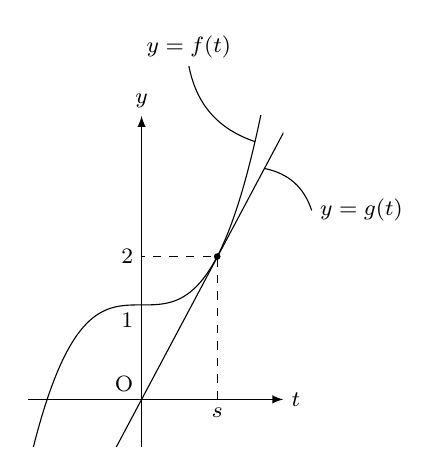
\begin{tikzpicture}[scale=1.2]
    %関数
    \begin{scope}
      \clip(-1.2,-0.5)rectangle(1.5,{3});
      \draw[samples=300]plot(\x,{pow(\x,3)+1});
      \draw plot(\x,{1.88*\x});
    \end{scope}
    %軸
    \draw[->,>=latex](-1.2,0)--(1.5,0)node[right]{$t$};
    \draw[->,>=latex](0,-0.5)--(0,3)node[above]{$y$};
    %node
    \node[above left]at(0,0){O};
    \node[below left]at(0,1){1};
    \draw[dashed]({1-0.2},0)node[below]{$s$}--({1-0.2},{0.6*0.6*0.6+1+0.3})--(0,{0.6*0.6*0.6+1+0.3})node[left]{2};
    \fill ({sqrt(144)/15},{(sqrt(144)/15)*(sqrt(144)/15)*(sqrt(144)/15)+1})circle(1pt);
    \draw (1.2,{1.2*1.2*1.2+1})to[bend left](0.5,{1.2*1.2*1.2+1.8})node[above]{$y=f(t)$};
    \draw (1.3,{1.88*1.3})to[bend left](1.8,2)node[right]{$y=g(t)$};
  \end{tikzpicture}
\end{center}
この図より,接点$t=s$で$y=f(t)$と$y=g(t)$が接するときが$\asta$の上限である.\\
$y=f(t)とy=g(t)$が接するとき,$「f(t)とg(t)の傾きが等しい」$ので,接点を$\p{s,f\p{s}}$とおくと,
\begin{align*}
  \begin{cases}
    f^\prime(s)=g^\prime(s)\\
    f(s)=g(s)
  \end{cases}&\doti\begin{cases}
    3s^2=3a^2\\
    s^3+2=3a^2s
  \end{cases}\\
  &\doti\begin{cases}
    s^2=a^2\\
    s^3+2=3s^3
  \end{cases}\\
  &\doti\begin{cases}
    s^2=a^2\\
    (s-1)(s^2+s+1)=0
  \end{cases}\\
  &\doti\begin{cases}
    s^2=a^2\\
    s=1
  \end{cases}
\end{align*}
$\yueni$上限値は,$a^2=1$\\
$\yueni$求める$a$の範囲は,
\begin{align*}
  \begin{cases}
    a^2\leq1\\
    a\geq0
  \end{cases}\doti\ans{0\leq a\leq1}
\end{align*}
\chu\quad 流石京都大学,答えが美しいですね....
\begin{thickitembox}
  {\ba{1$\bullet$3}\midashikakko{東工大}}
  $a,b$を正数とするとき,$\p{\dfrac{a^2+b^2}{2}}^{\frac12}と\p{\dfrac{a^3+b^3}{2}}^{\frac13}$の大小を比較せよ.
\end{thickitembox}
\hokukan\quad 大小の比較は次の3通りの考え方が鉄板です.覚えておくと良いでしょう.\\
\doichi\ans{比をとる}\\
\doni\ans{差を考える}\\
\dosan\ans{関数の単調性を使う}\\
\doshi$\ans{イェンセンの不等式（y=\log xの平均値）を使う}$\\
本問の場合,正数なので何乗しても大小関係が変わらないので,\doichi を考えるのが良さそうです.6乗すれば,簡単な関数になりそうなので.また,\ans{大小関係を自分で設定する}というのも
受験数学の大きなテーマです.本問では$a,b$の大小関係を考える必要がありますが$a,b$が対称なので,自分が都合の良いように大小関係を設定すればよいです.\\
\hokukai$A=\p{\dfrac{a^2+b^2}{2}}^{\frac12},B=\p{\dfrac{a^3+b^3}{2}}^{\frac13}$とおいて,$0<b\leq a$としても,$a,b$の対称性から,一般性を失わない.このとき,
$1\leq\dfrac{a}{b}$なので,$t=\dfrac{a}{b}$とおくと,$1\leq t\cdots\cdots\maruichi$で,
\begin{align*}
  \p{\dfrac{A}{B}}^6&=\dfrac{\p{\dfrac{a^2+b^2}{2}}^{3}}{\p{\dfrac{a^3+b^3}{2}}^2}\\
  &=\dfrac12\cdot\dfrac{\p{a^2+b^2}^3}{\p{a^3+b^3}^2}\\
  &=\dfrac12\cdot\dfrac{\B{\p{\frac{a}{b}}^2+1}^3}{\B{\p{\frac{a}{b}}^3+1}^2}\\
  &=\dfrac12\cdot\dfrac{\p{t^2+1}^3}{\p{t^3+1}^2}
\end{align*}
よって,$A$と$B$の大小関係は,$\maruichi$における$\p{t^2+1}^3と2\p{t^3+1}^2$の大小関係と一致する.\\
ここで,$f(t)=2\p{t^3+1}^2-\p{t^2+1}^3$とおくと,
\end{document}